\documentclass[tikz,border=5pt]{standalone}
\usepackage[utf8]{inputenc}
\usepackage[T1]{fontenc}
\usepackage{lmodern,amsmath,amssymb}
\usepackage[american]{circuitikz}
\usepackage{pgfplots}
\pgfplotsset{compat=1.18}
\usetikzlibrary{circuits.logic.US,positioning,calc,arrows.meta,patterns,shapes.geometric}
\definecolor{Primary}{HTML}{1F77B4}
\begin{document}
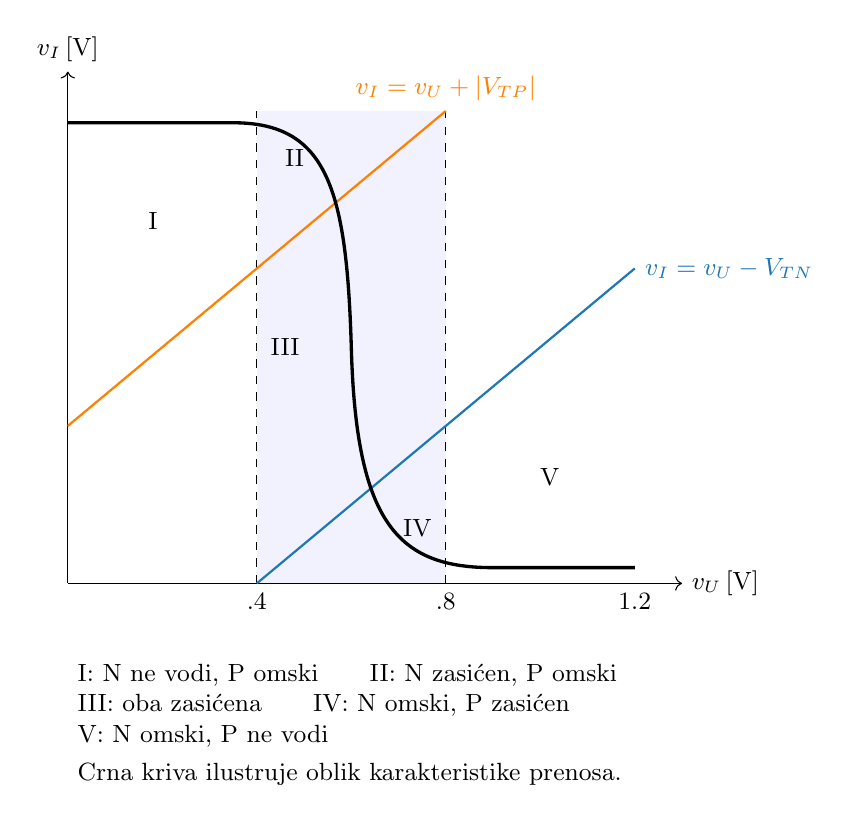
\begin{tikzpicture}[x=6cm,y=5cm,font=\small]
\fill[blue!5](.4,0)rectangle(.8,1.2);
\draw[->](0,0)--(1.3,0)node[right]{$v_U\,[\mathrm V]$};\draw[->](0,0)--(0,1.3)node[above]{$v_I\,[\mathrm V]$};
\draw[dashed](.4,0)--(.4,1.2)(.8,0)--(.8,1.2);
\draw[Primary,thick](.4,0)--(1.2,.8)node[right]{$v_I=v_U-V_{TN}$};
\draw[orange,thick](0,.4)--(.8,1.2)node[above]{$v_I=v_U+|V_{TP}|$};
\foreach\x in{.4,.8,1.2}\node[below]at(\x,0){\x};
\draw[black,very thick] (0,1.17)--(.35,1.17)
 .. controls (.55,1.17) and (.59,1.0) .. (.6,.6)
 .. controls (.61,.15) and (.7,.04) .. (.9,.04)--(1.2,.04);
\node at(.18,.92){I};
\node at(.48,1.08){II};
\node at(.46,.60){III};
\node at(.74,.14){IV};
\node at(1.02,.27){V};
\node[anchor=north west,align=left]at(0,-.18){%
 I: N ne vodi, P omski\qquad II: N zasićen, P omski\\
 III: oba zasićena\qquad IV: N omski, P zasićen\\
 V: N omski, P ne vodi\\[3pt]
 Crna kriva ilustruje oblik karakteristike prenosa.};
\end{tikzpicture}
\end{document}
